\documentclass[conference]{IEEEtran}
\usepackage{sidecap}
\usepackage[margin=0.75in]{geometry}
\usepackage{amsmath}
\usepackage{verbatim}
\usepackage{amssymb}
\usepackage{algorithm}
\usepackage{subfigure}
\usepackage{graphicx}
\usepackage[noend]{algpseudocode}
\usepackage{drum}
\usepackage{times}
\usepackage{url}

\usepackage{xspace}
\usepackage{color}
\newcommand{\todo}[1]{{\color{red}{\textbf{#1}}}\xspace}
\newcommand{\added}[1]{{\color{magenta}{#1}}\xspace}
\newcommand{\edited}[1]{{\color{blue}{#1}}\xspace}
\newcommand{\removed}[1]{{\color{red}{\sout{#1}}}\xspace}

% TODO: where does sustained contact model come from?

% numbers option provides compact numerical references in the text. 
\usepackage[numbers]{natbib}
\usepackage{multicol}
%\usepackage[bookmarks=true]{hyperref}

\author{John Shepherd, Samuel Zapolsky, and Evan M. Drumwright}
\title{
Fast Multi-Body Simulations of Robots Controlled with Error Feedback}

\sidecaptionvpos{figure}{c}

\newcounter{counthypothesis}
\newcommand{\hypothesis}[0]{\addtocounter{counthypothesis}{1}\textbf{Hypothesis \arabic{counthypothesis}: }}


\begin{document}
%\author{\authorblockN{Michael Shell}
%\authorblockA{School of Electrical and\\Computer Engineering\\
%Georgia Institute of Technology\\
%Atlanta, Georgia 30332--0250\\
%Email: mshell@ece.gatech.edu}
%\and
%\authorblockN{Homer Simpson}
%\authorblockA{Twentieth Century Fox\\
%Springfield, USA\\
%Email: homer@thesimpsons.com}
%\and
%\authorblockN{James Kirk\\ and Montgomery Scott}
%\authorblockA{Starfleet Academy\\
%San Francisco, California 96678-2391\\
%Telephone: (800) 555--1212\\
%Fax: (888) 555--1212}}


% avoiding spaces at the end of the author lines is not a problem with
% conference papers because we don't use \thanks or \IEEEmembership


% for over three affiliations, or if they all won't fit within the width
% of the page, use this alternative format:
% 
%\author{\authorblockN{Michael Shell\authorrefmark{1},
%Homer Simpson\authorrefmark{2},
%James Kirk\authorrefmark{3}, 
%Montgomery Scott\authorrefmark{3} and
%Eldon Tyrell\authorrefmark{4}}
%\authorblockA{\authorrefmark{1}School of Electrical and Computer Engineering\\
%Georgia Institute of Technology,
%Atlanta, Georgia 30332--0250\\ Email: mshell@ece.gatech.edu}
%\authorblockA{\authorrefmark{2}Twentieth Century Fox, Springfield, USA\\
%Email: homer@thesimpsons.com}
%\authorblockA{\authorrefmark{3}Starfleet Academy, San Francisco, California 96678-2391\\
%Telephone: (800) 555--1212, Fax: (888) 555--1212}
%\authorblockA{\authorrefmark{4}Tyrell Inc., 123 Replicant Street, Los Angeles, California 90210--4321}}


\maketitle

\begin{abstract}
Roboticists modeling control of manipulator and legged robots often  
assume force/torque-based control using an open-loop model of voltage, hydraulic
pressure, or pneumatic pressure to actuate torques. This work shows that such force/torque-based models can lead to stiff differential equations, which are computationally
inefficient to solve: relatively small integration steps are necessary to
ensure stability. 

We have investigated two approaches which appear to mitigate this problem: 
incorporating transmission modeling (applicable only to electromagnetic 
actuators at present) and applying inverse dynamics control. Both of these approaches require
increased computation per integration step, but this work will demonstrate that 
the larger integration steps can still yield considerably higher simulation 
throughput. 

This paper will also identify research challenges with using inverse dynamics 
control within multi-rigid body simulations. We examine a
state of the art approach concerning inverse dynamics control. We integrate the simulation subject to 
contact and inverse dynamics constraints, and we also identify algorithmic
challenges, both theoretical and practical. 
Experimental virtual robot platforms include a UR10 arm with attached prismatic manipulator and a
locomoting quadrupedal robot.
\end{abstract}

\section{Introduction}
Roboticists often wish to simulate controlled systems rapidly while prototyping
control schemes and hardware designs. In these cases, reducing the duration of 
the ``edit-compile-test'' cycle is more important than reducing numerical
solution error, which roboticists might do after obtaining some confidence 
in their approach. 

%As an anecdotal example of where such an approach might be useful, the last 
%author recently tasked students in a course with producing gait generation and 
%balance stabilization software for a simulated legged robot. The underactuated
%nature of the robot limited the utility of strictly kinematic simulation.
%And the inclusion of error feedback controllers, which requires careful
%tuning to balance dynamic performance with simulation stability, made debugging both more challenging (e.g., Did the robot fall because control was not
%sufficiently accurate?) and slower than desirable. With the inclusion of
%control, inverse kinematics, and planning code, simulations would run several
%times slower than real-time. 

%The present work continues a previous investigation~\cite{Zapolsky:2015} into 
%means to accelerate this process. That work found that exponential energy
%dissipation can be used to increase simulation stability. However, it should be clear
%that excessive dissipation will lead to artifacts (e.g., the robot acts as if
%it is moving through molasses), and we have found it challenging to balance numerical stability and physical fidelity with that approach. 
The present study started from the observation that simulating robots with few degrees of 
freedom and controlled via error feedback could admit large integration steps. These large integration steps can yield much faster simulations at the expense of lower numerical accuracy.
Accordingly, this paper tests the following hypotheses: 
  
\hypothesis Driving a multi-body system (e.g., a robot interacting through contact with one or more rigid bodies) through inverse dynamics control can yield greater numerical stability than tuned PD/PID control can offer. 

\hypothesis Integrating a multi-body system that accounts for both contact and inverse dynamics constraints yields greater numerical stability than feeding the output from an inverse dynamics controller into the simulation's integrator.

\hypothesis Incorporating transmission models for electromagnetic actuators can increase numerical stability for simulations of robotic systems driven by PD/PID control.





\begin{figure*}[htbp]
\centering
\subfigure[]{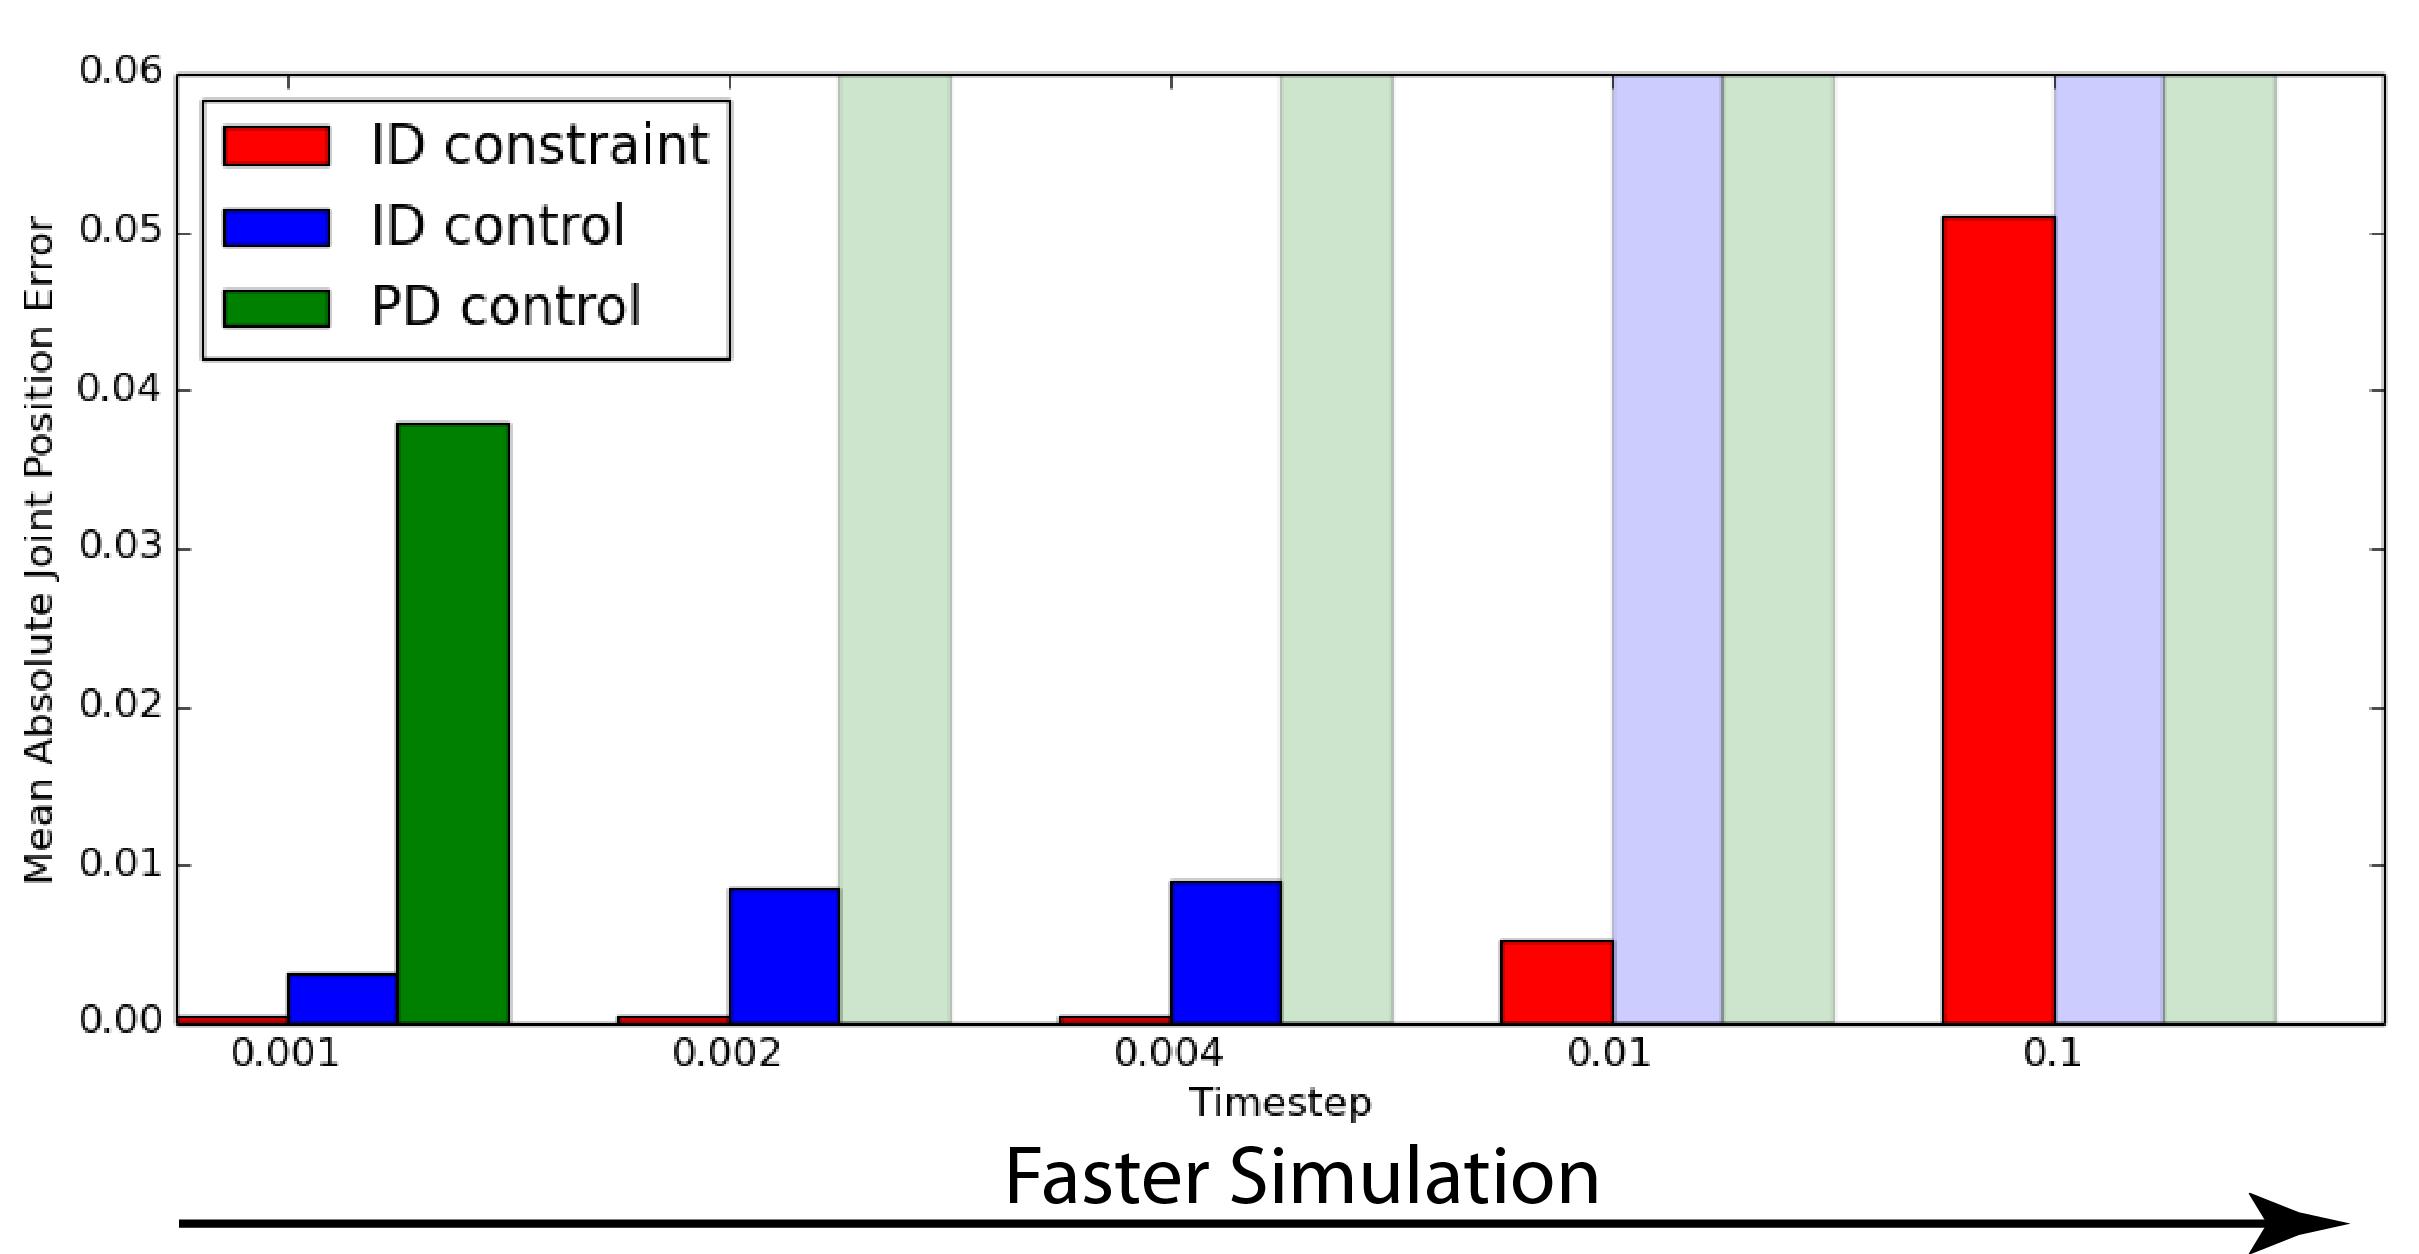
\includegraphics[height=1.75in]{Quad_pos2}}
\subfigure[]{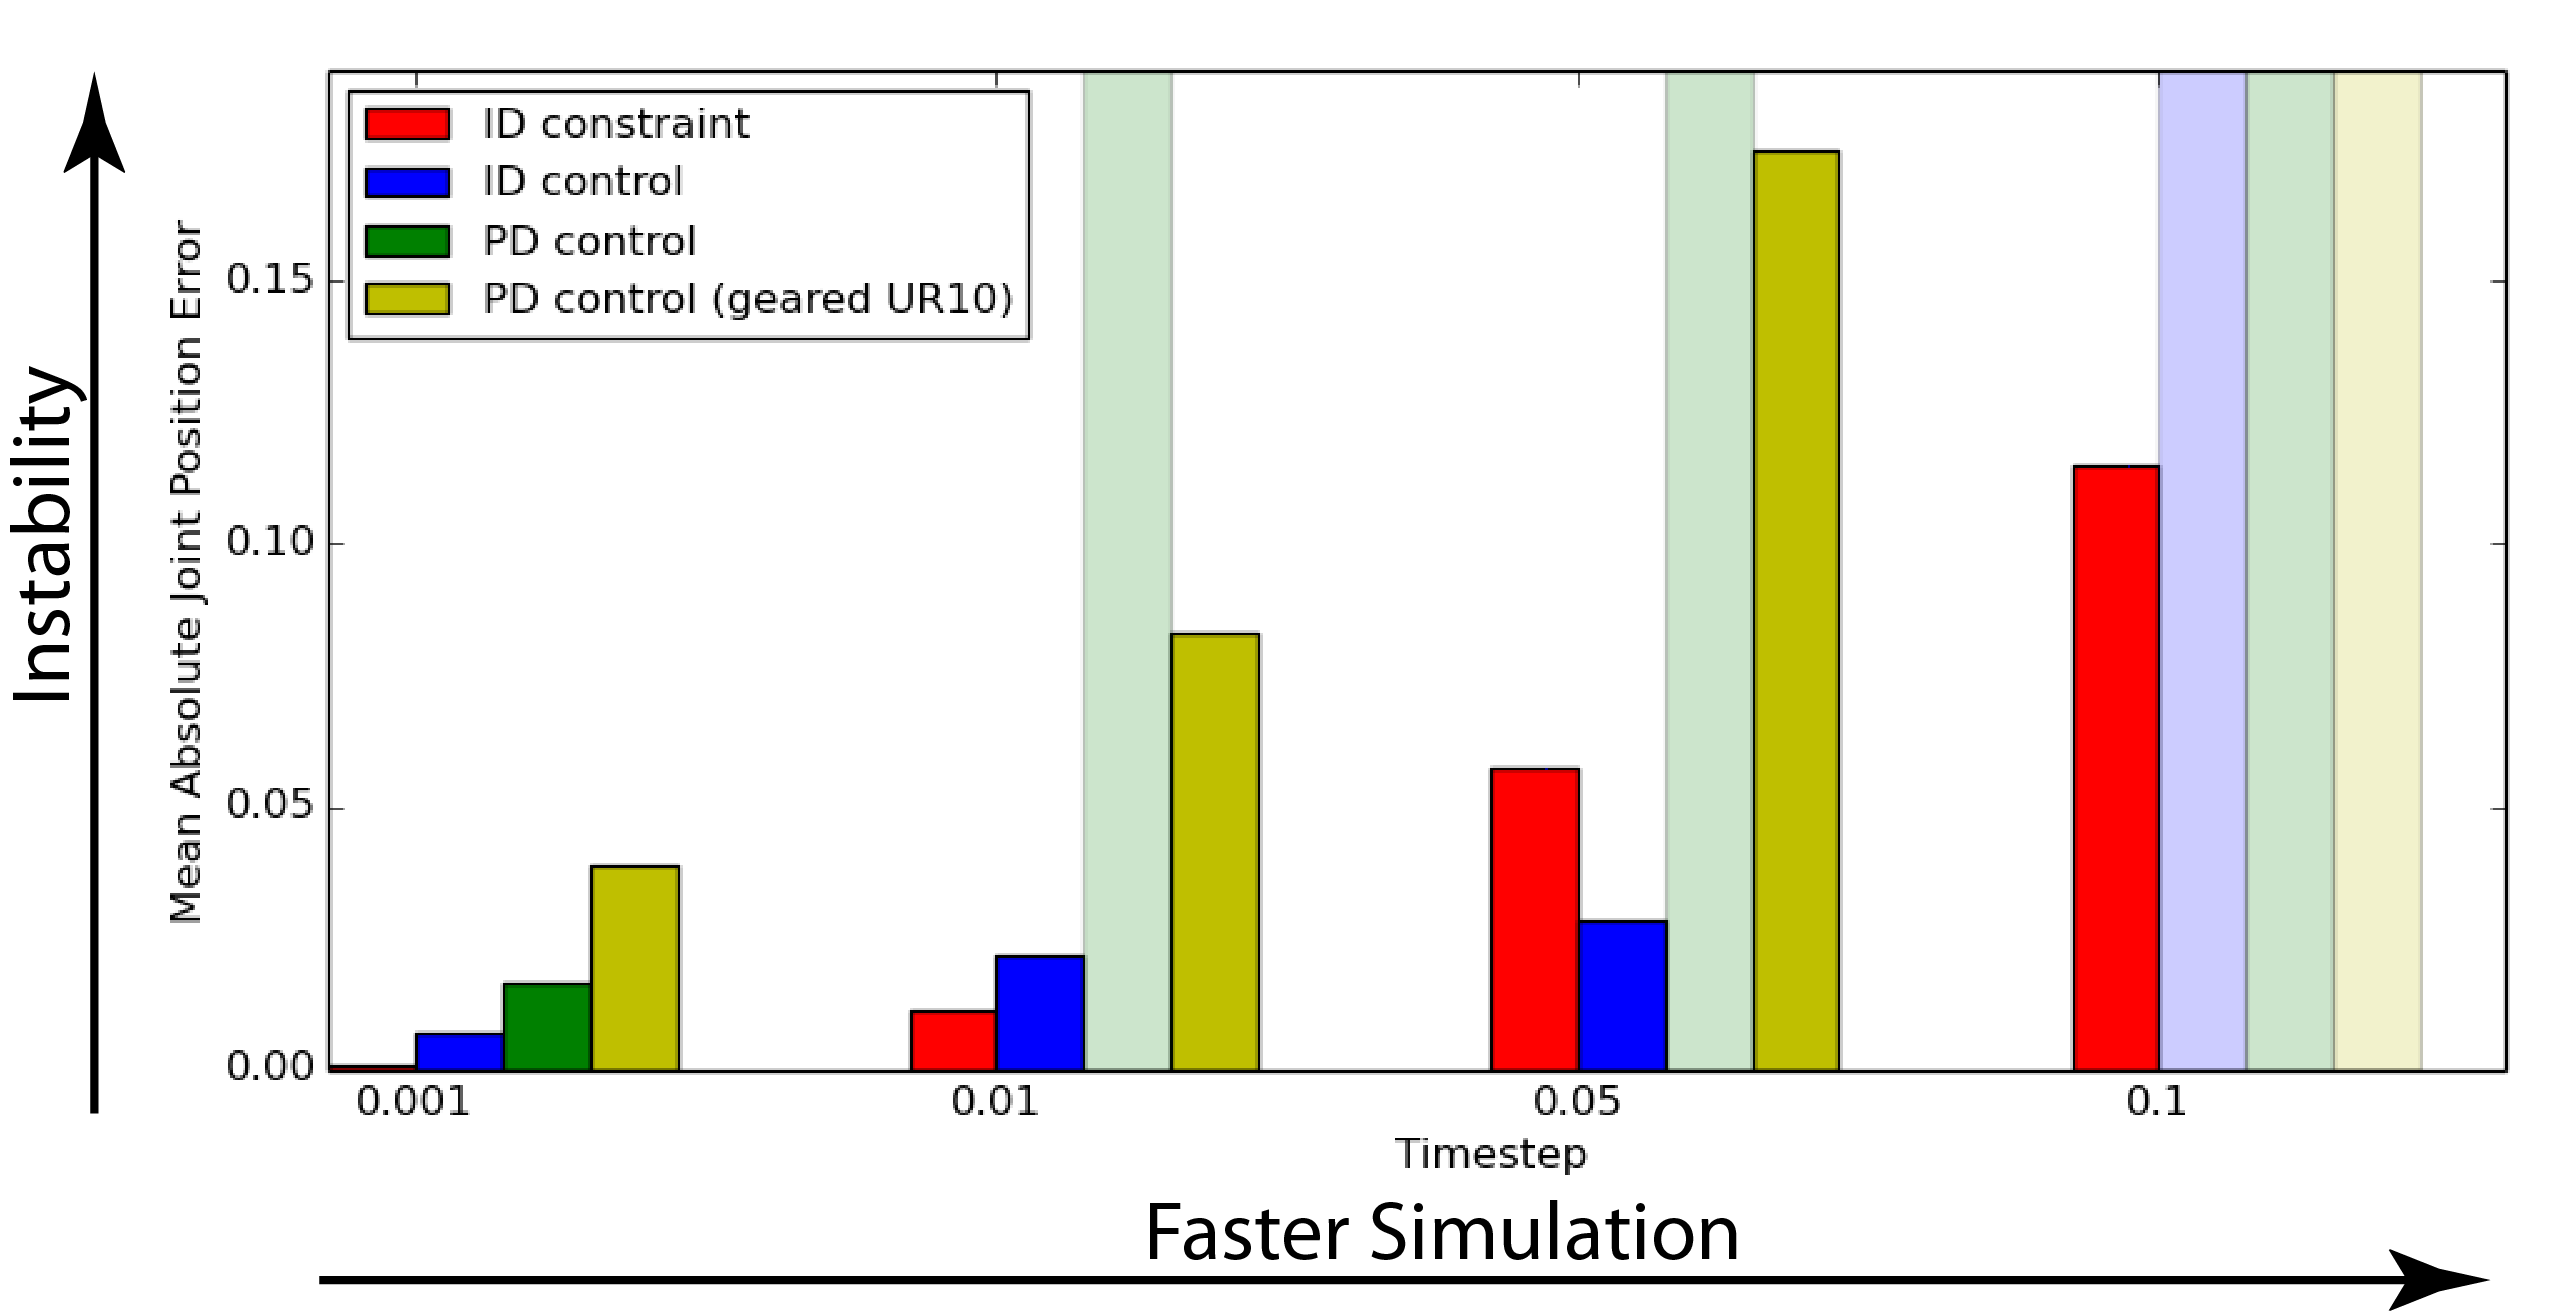
\includegraphics[height=1.75in]{UR10_pos2}}
\caption{(a). The mean absolute joint position error for the ID constraint, ID control, PD control and geared PD control for the UR10 at various timesteps.  A transparent bar indicates instability for the control at the given timestep.  Note that the PD control is unstable for all timesteps greater than 0.001.  The ID constraint controller is significantly more stable at orders of magnitude larger step sizes than the other controllers. It remains stable when the timestep is at the maximum tested 0.1.  The geared UR10 with PD control is able to achieve significantly higher timesteps than standard PD control at the cost of controller accuracy.}
\label{fig:pos_error}
\end{figure*}



\section{Experiments}

Simulation experiments were conducted using the multi-rigid body dynamics library \software{Moby}.  The robots used in the experiments were the UR10 arm (sourced from an existing open source ROS package), see Figure \ref{fig:UR10Arm}, and a floating base quadruped model described in existing work~\cite{Zapolsky:2015}.  The UR10 arm and attached prismatic manipulator, together, possess eight degrees-of-freedom (DoF), all controllable. The quadruped model possesses 18 DoF, 12 of which are controllable.

\begin{figure}[H]

\begin{center}
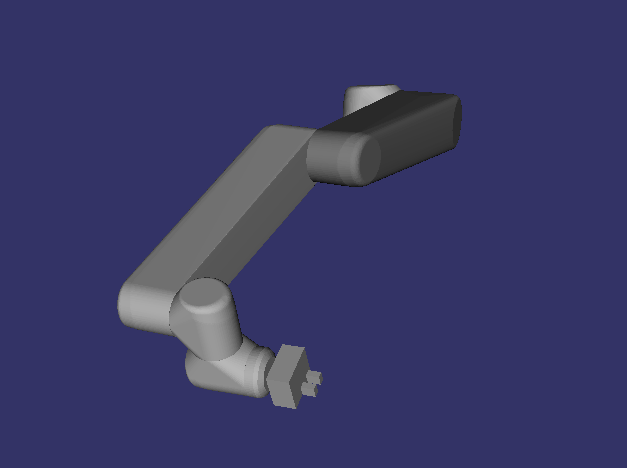
\includegraphics[scale=0.30]{UR10Arm.png}
\end{center}
\caption{The UR10 arm with attached prismatic gripper in simulation.\label{fig:UR10Arm}}
\end{figure}
For control testing, the UR10 was directed to follow a sinusoidal motion at each joint. %The desired joint angles set for each joint across time were a function of sine so the desired trajectory across each joint is sinusoidal. Each simulation was run for five seconds of virtual time.
A PD control was used in these experiments, and the gains for the control were tuned by a two-part process consisting of manual tuning followed by nonlinear optimization. The gains were tuned in this way to eliminate human bias to the greatest extent possible. 

%Where applicable, our experiments use inverse dynamics-based algorithms that \emph{can} account for torque limits---the ones described in this paper, not~\cite{Zapolsky:2015c}---even though torque limits are set to $\pm \infty$ (i.e., unused). This decision allowed us to study the computational properties of these methods without focusing on whether our virtual robots would possess the actuator forces necessary to complete tasks.
Integration steps were limited, albeit arbitrarily, to a maximum of $0.1$s. The initial integration step size tested for each model was $0.001$, a value that we confirmed produced stable simulations of each model readily. Step sizes were doubled until instability resulted.%---at which point bisection search was conducted to identify an approximate maximum stable step size---or the maximum value of $0.1$s was reached.


\subsection{Testing Hypothesis 1: incorporating inverse dynamics control leads to more stable simulations than error feedback control}

A PD-controlled UR10 arm served as one experimental control for Hypothesis~1. The maximum step size we attained using this controller without the simulation becoming unstable was $0.001$. On the other hand, we found that we could simulate the UR10 arm stably without any controls applied (i.e., the robot falls under the influence of gravity) with a step size of $0.1$. An experimental control in a second experiment used the quadrupedal robot model driven by PD control. 
% \emph{This result indicates that the PD control introduces stiffness into the differential equations}; this result is not surprising given that \1 PD control can be viewed as a virtual spring damper and \2 the mass-spring system is the canonical example of a stiff ordinary differential equation~\cite{Hairer:1996}. For the experimental variable, we used the standard recursive Newton-Euler Algorithm~\cite{Featherstone:1987} to generate inverse dynamics torques.

%We used the non-complementarity-based inverse dynamics control approach described in~\cite{Zapolsky:2015c}, which was necessary since one or more links of the robot remained in contact with the environment, as our experimental variable. Tables~\ref{table:quad}~and~\ref{table:UR10} list the results from the experiments with both robots: inverse dynamics control allows the simulations to run 500\% and 5480\% faster, respectively.


In both experiments, the ID control was able to achieve a higher timestep than the PD control. Figure~\ref{fig:pos_error} (a) shows that during the quadruped experiment, the ID control was able to achieve a maximum stable timestep of 0.004. The PD control, on the other hand was only able to achieve a maximum timestep of 0.001. Part (b) shows the ID control being able to achieve a timestep of 0.05 when the sinusoidal motion was run on the UR10 arm.  PD control was still only able to achieve a maximum step size of 0.001.  %The large increase of timestep with regards to the ID control from the quadruped experiment to the UR10 experiment is likely due to the fact that the quadruped actually experiences contact in its controlled motion, while the UR10 experiences no contact.

\subsection{Testing Hypothesis 2: incorporating inverse dynamics constraints leads to more stable simulations than using inverse dynamics control}
\label{section:hypo2}


%Hypothesis~2 arose from our observations about the split nature of the control-simulation process: we speculated that solving for the next velocity subject to all constraints would yield higher greater simulation stability than feeding the inverse dynamics torques into the simulator's constraint solver. 

We used the inverse dynamics controllers employed as the experimental variables in our tests of Hypothesis~1 as the experimental controls in our tests of Hypothesis~2. For the variables in this experiment, we tested the UR10 arm and the quadrupedal robot. We also tested the quadrupedal robot using an experimental, optimization-based constraint solver. 

For the UR10 at a timestep of 0.01, the use of inverse dynamics constraints is able to achieve around the same order of accuracy as the PD control at a timestep of 0.001. Incorporating ID constraints into the UR10 simulation process executed in 2.85s at a 0.01 timestep, while the PD controlled arm required 357.02s at a 0.001 timestep. ID constraints achieved a 125x speedup with essentially the same accuracy.

%The results for the quadrupedal robot in Table~\ref{table:quad} require explanation. The existing, MLCP-based approach caused the simulation to become unstable at any step size. Regularizing the MLCP (via Tikhonov regularization) did not help: such large regularization---it was necessary to add values on the order of $1.0$ to MLCP matrix to attain a solution---that the result was no longer a solution to a ``nearby'' problem. Note that applying the constraint solver to the individual problems of inverse dynamics without contact (by temporarily de-activating gravitational forces) and contact without inverse dynamics (i.e., just using PD control) works fine; problems only arise when the constraints are considered simultaneously. We used the Dantzig solver~\cite{Lacoursiere:2007}, which is also used by \software{ODE}, to solve the mixed linear complementarity problem. 

%Our experimental approach outlined above was capable of generating an accurate solution---and, as with the UR10 model---the simulation remained perfectly stable for large step sizes. However, our results do not capture an important artifact: the quadruped appeared to be skating as if on ice when it should have been trotting.  Examination of the constraint solver indicated that the solution method would have had to slightly violate the inverse dynamics constraints to incorporate frictional forces; our experimental approach is flawed and thus illustrates what can happen when constraints may be violated arbitrarily. 


\subsection{Testing Hypothesis 3: incorporating transmission models increases the stability of robots driven by error feedback control}
Claude Lacoursi\`{e}re suggested in personal communication that adding gearing to a robot model might reduce the stiffness in the differential equations. Accordingly, we compared the PD controlled UR10 used to test Hypothesis~1 to a PD controlled UR10 with a virtual transmission modeled at each revolute joint; the gains were re-tuned for this modified model.  Gearing was not added to our quadrupedal model because significant architectural modifications would be necessary in our robot's locomotion software to accommodate gearing. Data did indicate that the gearing does dramatically increase the maximum stable step size, at a clear cost of tracking accuracy.

\section{Discussion}

We have demonstrated the capability of inverse dynamics to dramatically speed multi-rigid body simulations with contact.  In our experiments, the maximum stable integration step sizes were tens or hundreds of times larger, thereby permitting much faster simulations.  We have also shown that incorporating constraints into the constraint solver for control is less likely to cause simulation instability. %We believe that the explanation for the stability decrease by feeding the inverse dynamics forces/torques into the simulation is due to very slight discrepancies in inputs. %Our prior work~\cite{Zapolsky:2015c}, which demonstrates high, although imperfect tracking accuracy for inverse dynamics of simulated robots, hints at this phenomenon. 

It is clear that important work still remains, particularly in finding a computationally tractable model that produces reasonably accurate contact forces and satisfies inverse dynamics constraints as well as force/torque limits. In the meantime, adding gearing to robots with electromagnetic actuators can provide the requisite simulation stability necessary for high frequency (realtime and above) simulation, albeit with far lower tracking accuracy.


%\begin{figure}[htpb]
%\begin{tabular}{ |p{3cm}||p{1cm}|p{1cm}|p{1cm}|p{1cm}| }
%\hline
%\multicolumn{5}{|c|}{Runtimes of Controllers (UR10) in seconds}\\
%\hline
%Controller Type& 0.001&0.01&0.05&0.10\\

%\hline
%ID&196.75&23.38&6.157&--\\
%ID constraint{$^{*}$}&72.29&9.11&3.54&2.85\\
%PD&357.02&--&--&--\\
%Geared PD&905.74&96.92&24.56&--\\

%\hline
%\end{tabular}
%\caption{* The ID constraint controller ran the fastest across all timesteps.}
%\end{figure}
%\begin{figure}
%\begin{tabular}{ |p{4cm}||p{1cm}|p{1cm}|p{1cm}|p{1cm}| }
%\hline
%\multicolumn{4}{|c|}{Runtimes of Controllers (Quadruped) in seconds}\\
%\hline
%Controller Type& 0.001&0.01&0.10\\
%\hline
%ID&18.38&--&--\\
%ID constraint &85.375&13.34&2.54\\
%PD &16.20&--&--\\

%\hline
%\end{tabular}
%\caption{* The ID constraint controller ran the fastest across all timesteps.}
%\end{figure}

\bibliographystyle{abbrv}
\bibliography{paper}

\end{document}


